\section{Warlock Class Weapons}

\subsubsection{Spine of the Condemned}

According to legend, a powerful warlock named Kael'thas teamed up with a powerful Wizard named Xavius in studying alternate realms and dimensions. Kael'thas opened a portal to a demonic realm and saught the power that the creatures within it possessed. In an attempt to control the beings from that realm, he trapped their souls in a magical crystal. The crystal contained the essence of the creatures but the power was unable to be used until Xavius crafted a staff to connect with the power of the crystal. Unfortunately, with the dark ways of Xavius' sorcery, the process required a trusting soul, in which Kael'thas was consumed to the staff. Later named the Spine of the Condemned, it is said that Kael'thas' essence is trapped within the soul and along with its wielder, can tap the potential of the demonic souls that are contained within the Spines crystal. The great Wizard Xavius is legend to have gone mad from his own creations and lose all knowledge of his magical creations. The Spine of the Condemned is said to have vanished along with all of his other dark creations of the time.

\begin{center}
	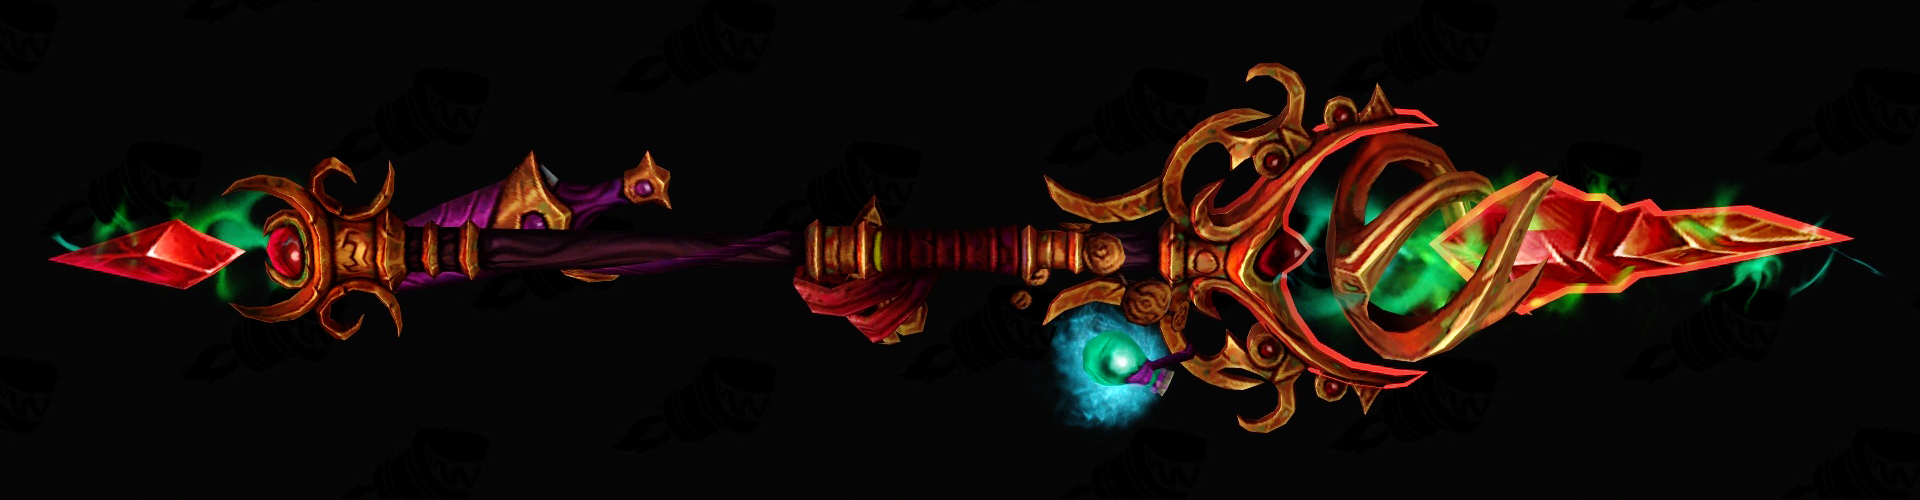
\includegraphics[width=\linewidth]{img/weapons/532325-ebonchill-fire-mage-artifact.jpg}
\end{center}

\subsubsection{Potential}

The Spine of the Condemned seeks to release its power within the hands of a powerful warlock. 

\begin{commentbox}{Spine of the condemned\footnote{Weapon (staff), artifact (requires attunement by a warlock)}}
	You gain a +3 bonus to attack and damage rolls made while wielding this magic weapon. 
	
	When attuned to this staff, the wielder can communicate with Kael'thas and spend 1 minute to summon one of the trapped demonic spirits contained within the staff to serve the wielder. The creature summoned can be any of those in the below list based on the maximum level of the wielding warlock. The summoned creature rolls initiative and has its own turn.
	\begin{multicols}{4}
		\begin{itemize}
			\item lvl 1+: Imp Fiend.
			\item lvl 4+: Voidwalker. 
			\item lvl 7+: Succubus.
			\item lvl 10+: Felhunter. 
			\item lvl 13+: Felguard.
			\item lvl 16+: Doomguard.
			\item lvl 19+: Infernal.
		\end{itemize}
	\end{multicols}
	
	Proficiency with a staff allows you to add your proficiency bonus to the attack roll for attacks you make with it.
	
	\begin{center}
		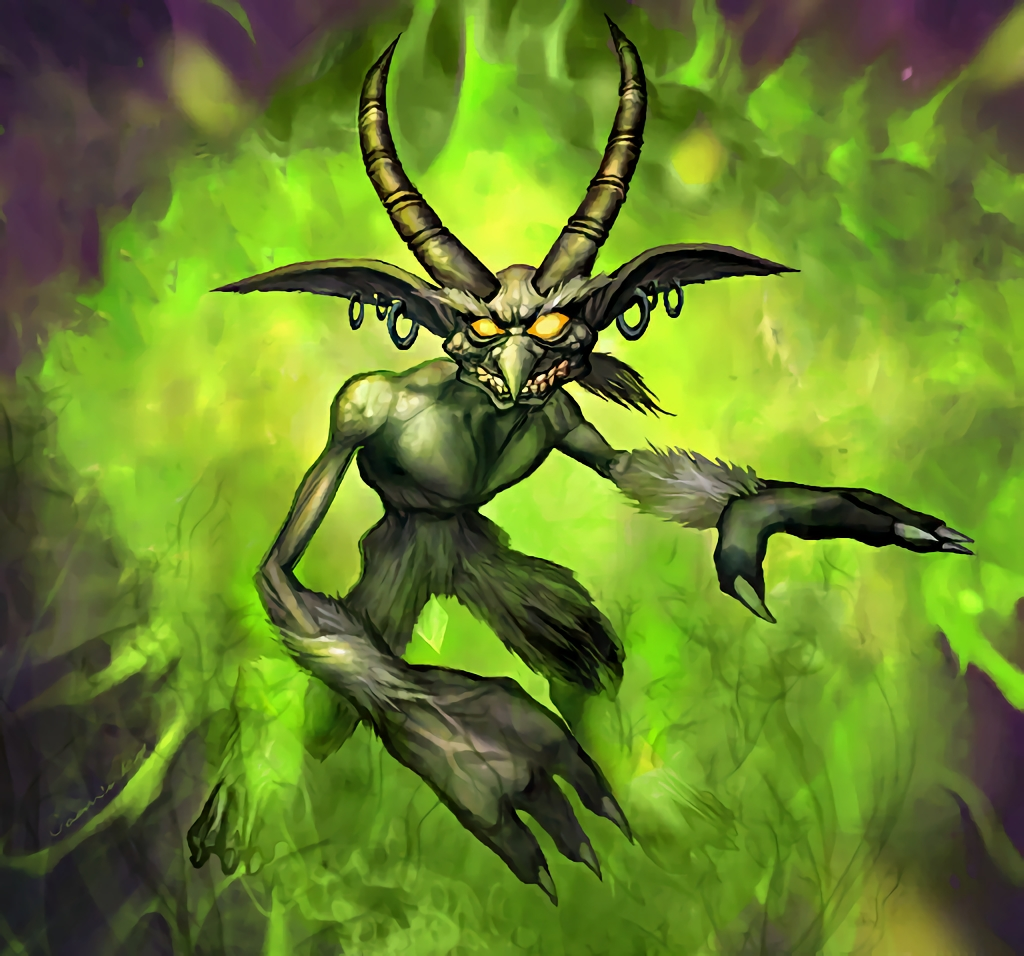
\includegraphics[width=0.355\linewidth]{img/WoW/ImpHS.jpg} 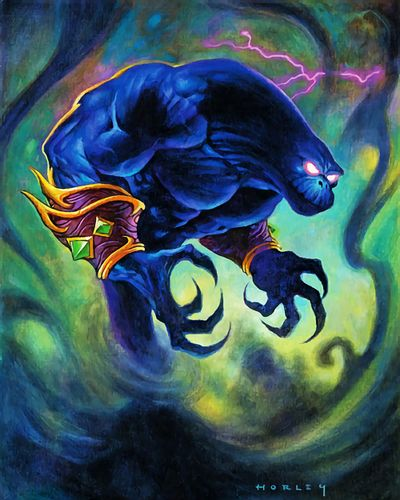
\includegraphics[width=0.265\linewidth]{img/WoW/400px-Voidwalker(art).jpg}
		%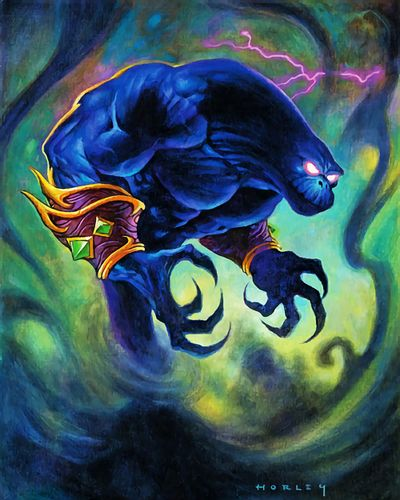
\includegraphics[width=0.21\linewidth]{img/WoW/400px-Voidwalker(art).jpg}
		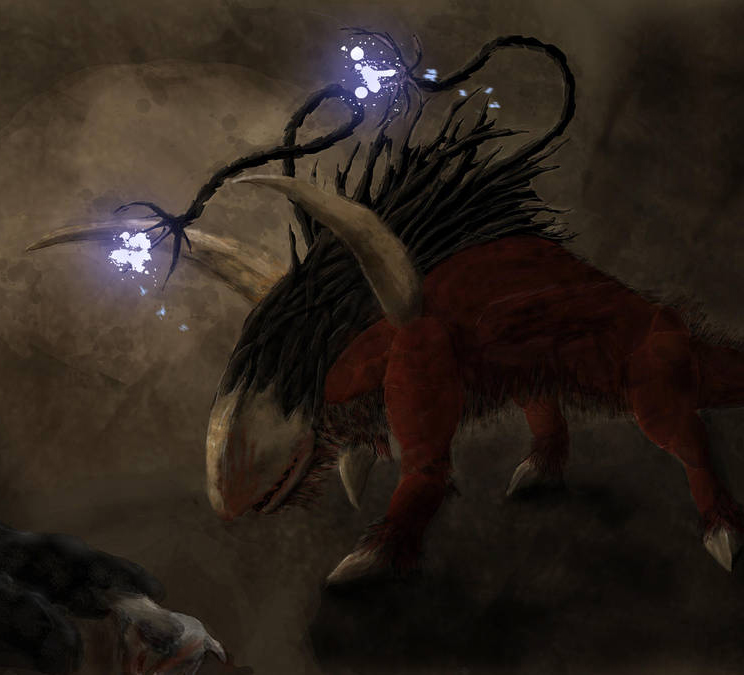
\includegraphics[width=0.365\linewidth]{img/WoW/felhunterart.jpg}
		
		Imp \hspace{4cm} Voidwalker \hspace{3.5cm} Felhunter
	\end{center}
	\begin{center}
		
\includegraphics[width=0.52\linewidth]{img/WoW/516px-Felguard-art.jpg}
		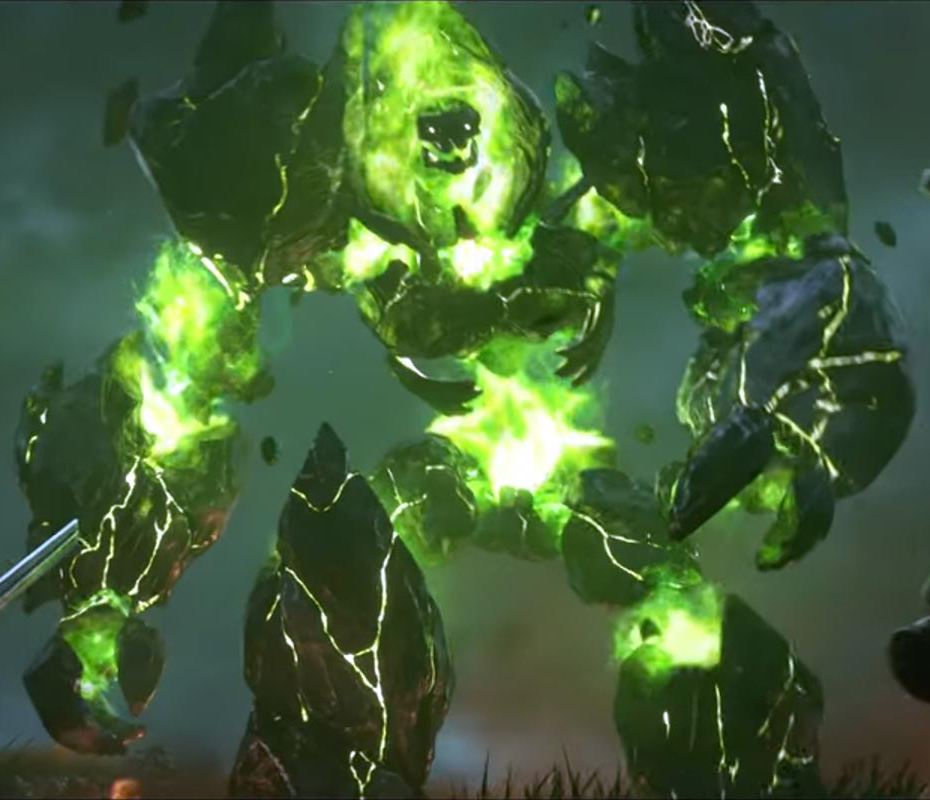
\includegraphics[width=0.47\linewidth]{img/WoW/Warcraft-III-Reforged-Cinematic-Trailer.jpg}
		
		Felguard \hspace{7.5cm} Infernal
	\end{center}
\end{commentbox}

\begin{monsterbox}{Imp}
	\begin{hangingpar}
		\textit{Tiny fiend (demonoid), lawful evil}
	\end{hangingpar}
	\dndline%
	\basics[armorclass = 13, hitpoints = 10 + summoners level, speed = 20 ft]
	\dndline%
	\stats[STR = \stat{6}, DEX = \stat{17}, CON = \stat{13}, INT = \stat{11}, WIS = \stat{12},	CHA = \stat{14}]
	\dndline
	languages = {demonic}
	]
	
	\dndline%
	damage immunities = Poison
		
	Senses = Darkvision 60 ft., passive Perception 11
	
	\dndline%
	\begin{monsteraction}[Devil's Sight]
		Magical Darkness doesn't impede the imp's Darkvision.
	\end{monsteraction}	
	\begin{monsteraction}[Magic Resistance]
		The imp has advantage on Saving Throws against Spells and other magical Effects.
	\end{monsteraction}	
	\begin{monsteraction}[Blood Bond of Kael'thas]
		You have a pact to serve the controller of the Spine of the Condemned
	\end{monsteraction}	
	\monstersection{Actions}
	\begin{monsteraction}[Sting (Bite)]
		Melee Weapon Attack: +5 to hit, reach 5 ft., one target. Hit: (1d4 + 3) piercing damage plus (1d4) poison damage. The poison damage dice increases by one based on the summoners level at levels 5, 11, and 17.
	\end{monsteraction}	
	\begin{monsteraction}[Poison Bolt (cantrip)]
		You hurl a small flame at a creature or object, making a ranged spell attack. The target takes 1d10 poison damage on hit. The spell's number of damage dice increases by one based on the summoners level at levels 5, 11, and 17.
	\end{monsteraction}	
\end{monsterbox}

\begin{monsterbox}{Voidwalker}
	\begin{hangingpar}
		\textit{medium shadow fiend (demonoid), lawful evil}
	\end{hangingpar}
	\dndline%
	\basics[armorclass = summoners AC +3, hitpoints = 30 + 4 $\times$ player level, speed = 30 ft]
	\dndline%
	\stats[STR = \stat{19}, DEX = \stat{12}, CON = \stat{18}, INT = \stat{10}, WIS = \stat{10},	CHA = \stat{10}]
	\dndline
	languages = {demonic, abyssal}
	]
	
	\dndline%
	damage immunities = psychic
	
	Senses = Darkvision 60 ft., passive Perception 10
	
	\dndline%
	\begin{monsteraction}[Dark Sense]
		When in a completely dark area, the voidwalker can sense its surroundings as if it could see perfectly.
	\end{monsteraction}	
	\begin{monsteraction}[Magic Resistance]
		The voidwalker has advantage on Saving Throws against Spells and other magical Effects.
	\end{monsteraction}	
	\begin{monsteraction}[Blood Bond of Kael'thas]
		You have a pact to serve the controller of the Spine of the Condemned
	\end{monsteraction}	
	\monstersection{Actions}
	\begin{monsteraction}[Slash (melee claw attack)]
		Melee Weapon Attack: +5 to hit, reach 5 ft., one target. Hit: (1d6 + 4) slashing damage plus (1d6) psychic damage. The psychic damage dice increases by one based on the summoners level at levels 5, 11, and 17.
	\end{monsteraction}	
\end{monsterbox}

\begin{monsterbox}{Succubus}
	\begin{hangingpar}
		\textit{small-medium fiend (demonoid), lawful evil}
	\end{hangingpar}
	\dndline%
	\basics[armorclass = summoners AC, hitpoints = 20 + 2 $\times$ player level, speed = 30 ft]
	\dndline%
	\stats[STR = \stat{8}, DEX = \stat{17}, CON = \stat{13}, INT = \stat{15}, WIS = \stat{12},	CHA = \stat{20}]
	\dndline
	languages = {demonic, abyssal, infernal}
	]
	
	\dndline%
	skills = Deception +9, Persuasion +9
	
	Senses = Darkvision 30 ft., passive Perception 11
	
	\dndline%
	\begin{monsteraction}[Telepathic Bond]
		The fiend ignores the range restriction on its telepathy when communicating with a creature it has charmed. The two don't even need to be on the same plane of existence.
	\end{monsteraction}	
	\begin{monsteraction}[Blood Bond of Kael'thas]
		You have a pact to serve the controller of the Spine of the Condemned
	\end{monsteraction}	
	\monstersection{Actions}
	\begin{monsteraction}[Claw (melee claw attack)]
		Melee Weapon Attack: +5 to hit, reach 5 ft., one target. Hit: (1d6 + 3) slashing damage. 
	\end{monsteraction}	
	\begin{monsteraction}[Charm]
		 One humanoid the fiend can see within 30 feet of it must succeed on a DC 15 Wisdom saving throw or be magically charmed for 1 day. The charmed target obeys the fiend's verbal or telepathic commands. If the target suffers any harm or receives a suicidal command, it can repeat the saving throw, ending the effect on a success. If the target successfully saves against the effect, or if the effect on it ends, the target is immune to this fiend's Charm for the next 24 hours. The fiend can have only one target charmed at a time. If it charms another, the effect on the previous target ends.
	\end{monsteraction}	
	\begin{monsteraction}[Draining Kiss]
 		The fiend kisses a creature charmed by it or a willing creature. The target must make a DC 15 Constitution saving throw against this magic, taking 32 (5d10 + 5) psychic damage on a failed save, or half as much damage on a successful one. The target's hit point maximum is reduced by an amount equal to the damage taken. This reduction lasts until the target finishes a long rest. The target dies if this effect reduces its hit point maximum to 0.
	\end{monsteraction}	
\end{monsterbox}

\begin{monsterbox}{Felhunter}
	\begin{hangingpar}
		\textit{medium fiend (demonoid), lawful evil}
	\end{hangingpar}
	\dndline%
	\basics[armorclass = 15, hitpoints = 30 + 3 $\times$ player level, speed = 50 ft]
	\dndline%
	\stats[STR = \stat{17}, DEX = \stat{12}, CON = \stat{14}, INT = \stat{6}, WIS = \stat{13},	CHA = \stat{6}]
	\dndline
	languages = {demonic}
	]
	
	\dndline%
	
	skills = Perception +6
	
	damage immunities = lightning
	
	senses = blind, passive Perception 12
	
	\dndline%
	\begin{monsteraction}[Keen hearing and Smell]
		The hound has advantage on Wisdom (Perception) checks that rely on hearing or smell.
	\end{monsteraction}	
	\begin{monsteraction}[Magic Resistance]
		The felhunter has advantage on Saving Throws against Spells and other magical Effects.
	\end{monsteraction}	
	\begin{monsteraction}[Blood Bond of Kael'thas]
		You have a pact to serve the controller of the Spine of the Condemned
	\end{monsteraction}	
	\monstersection{Actions}
	\begin{monsteraction}[Bite]
		Melee Weapon Attack: +5 to hit, reach 5 ft., one target. Hit: (1d8 + 3) piercing damage plus (3d6) lightning damage. The fire damage dice increases by one based on the summoners level at levels 11, and 17.
	\end{monsteraction}	
	\begin{monsteraction}[Devour Magic]
		You can use your action to devour nearby magic. You can also use this action to ready yourself so that you can intercept a single target magical attack before your next turn. To do so you must succeed a DC10 dexterity save. You take no damage from this magical attack that you devour.
	\end{monsteraction}	
\end{monsterbox}

\begin{monsterbox}{Felguard}
	\begin{hangingpar}
		\textit{large fiend (demonoid), lawful evil}
	\end{hangingpar}
	\dndline%
	\basics[armorclass = 16 Plate, hitpoints = 50 + 3 $\times$ player level, speed = 50 ft]
	\dndline%
	\stats[STR = \stat{24}, DEX = \stat{18}, CON = \stat{24}, INT = \stat{12}, WIS = \stat{13},	CHA = \stat{19}]
	\dndline
	languages = {demonic, abyssal, infernal}
	]
	
	\dndline%
	
	saving throws = strength +10, constitution +10

	condition immunities =  Blinded, Charmed, Deafened, Frightened, Petrified 
	
	senses = passive Perception 15
	
	\dndline%
	\begin{monsteraction}[Savage attacks]
		When the Felguard crits, it does triple dmg
	\end{monsteraction}	
	\begin{monsteraction}[Blood Bond of Kael'thas]
		You have a pact to serve the controller of the Spine of the Condemned
	\end{monsteraction}	
	\monstersection{Actions}
	\begin{monsteraction}[Axe]
		Melee Weapon Attack: +4 to hit, reach 10 ft., 1 target. Hit: 29 (6d6 + 7) slashing damage. 
	\end{monsteraction}	
	\begin{monsteraction}[Cleave (recharge 6)]
		Melee weapon attack: +4 to hit, reach 10 ft, multiple targets. All targets in a 10 ft radius sphere centered around the Felguard receive an Axe attack.
	\end{monsteraction}	
	\begin{monsteraction}{Charge}
		The Felguard moves up to its speed and makes an Axe attack. 
	\end{monsteraction}
\end{monsterbox}

\subsubsection{Finding the Spine of the Condemned}